% =====================================================================
%  Channel-realism audit of semantic communication for NTN
%  Dich: Computer Networks (Elsevier, hybrid, KHONG gold OA)
%
%  ⛔ KHONG GO SO. Moi con so den tu figures/out/numbers.tex, sinh tu results/*.json.
%     Chay: python3 code/e1_orbital_reality.py && python3 figures/make_figures.py
%
%  ⛔ RANG BUOC TU claim-structure.md, giu nguyen khi sua:
%   - KHONG duoc noi linh vuc nay "cau tha". Khao sat CO cot channel consideration.
%   - KHONG duoc de xuat chi so danh gia moi (khe do da bi arXiv:2608.21626 chiem).
%   - KHONG duoc ban lai luan diem "baseline co dien yeu" (khe da kin).
%   - PHAI bao ra ket qua SNR troi cham, vi no BENH VUC van lieu.
% =====================================================================
\documentclass[preprint,11pt,3p]{elsarticle}

\usepackage[T1]{fontenc}
\usepackage[utf8]{inputenc}
\usepackage{graphicx}
\usepackage{booktabs}
\usepackage{amsmath,amssymb}
\usepackage{url}
\usepackage[hidelinks]{hyperref}

%% SINH TU DONG boi figures/make_figures.py. KHONG SUA TAY.
%% Chi ASCII: tep nay duoc nap boi ca main.tex lan cac tep hinh
%% standalone, va mot so tep hinh khong nap inputenc.
\newcommand{\numCoded}{26}
\newcommand{\numDopKaMax}{455.5}
\newcommand{\numDopKaMed}{359.2}
\newcommand{\numDopRate}{5.4}
\newcommand{\numDopRateMax}{16.9}
\newcommand{\numDopS}{35.9}
\newcommand{\numDopSpread}{15.6}
\newcommand{\numDurMax}{285.5}
\newcommand{\numDurMed}{206.0}
\newcommand{\numEvATMOS}{6}
\newcommand{\numEvCHAWGN}{16}
\newcommand{\numEvCHFADING}{8}
\newcommand{\numEvCHGPP}{4}
\newcommand{\numEvCHTRACE}{0}
\newcommand{\numEvDELAY}{8}
\newcommand{\numEvDOPPLER}{11}
\newcommand{\numEvDOPPLERRATE}{0}
\newcommand{\numEvONBOARD}{3}
\newcommand{\numEvPATHLOSSELEV}{9}
\newcommand{\numEvSNRSWEEP}{7}
\newcommand{\numEvVISIBILITY}{3}
\newcommand{\numFsplMax}{6.72}
\newcommand{\numFsplMed}{3.72}
\newcommand{\numFull}{27}
\newcommand{\numFullPct}{58.7}
\newcommand{\numInATMOS}{2}
\newcommand{\numInCHAWGN}{1}
\newcommand{\numInCHFADING}{0}
\newcommand{\numInCHGPP}{0}
\newcommand{\numInCHTRACE}{0}
\newcommand{\numInDELAY}{4}
\newcommand{\numInDOPPLER}{2}
\newcommand{\numInDOPPLERRATE}{0}
\newcommand{\numInONBOARD}{3}
\newcommand{\numInPATHLOSSELEV}{1}
\newcommand{\numInSNRSWEEP}{2}
\newcommand{\numInVISIBILITY}{2}
\newcommand{\numNotFull}{19}
\newcommand{\numOwd}{3.25}
\newcommand{\numPasses}{30,922}
\newcommand{\numPassesStation}{1,978}
\newcommand{\numPop}{46}
\newcommand{\numSats}{1,200}
\newcommand{\numSlew}{0.049}
\newcommand{\numSlewTen}{0.49}


\journal{Computer Networks}

\begin{document}

\begin{frontmatter}

\title{Evaluated Under What? A Channel-Realism Audit of Semantic\\
Communication for Non-Terrestrial Networks}

\author[a]{Anonymous}
\address[a]{Affiliation withheld for review}

\begin{abstract}
Semantic communication is recommended for non-terrestrial networks on the argument that it
tolerates the conditions those links impose: large propagation delay, Doppler shifts of hundreds
of kilohertz, short visibility windows and an elevation-dependent link budget. Surveys of the
area map each of these limitations onto the works said to address it. We ask the narrower
question those mappings leave open, namely whether the works cited as addressing a limitation are
evaluated under it. Two measurements answer it. First, propagating \numSats{} public Starlink
two-line element sets with SGP4 over \numPasses{} passes fixes the magnitude of each effect from
orbital geometry rather than from assumption: peak Doppler reaches \numDopKaMed~kHz at Ka-band
with a drift of up to \numDopRateMax~kHz/s, and the geometric term of the link budget sweeps
\numFsplMed~dB across a median visibility window of \numDurMed~s. Second, a coding of the
\numPop{} works a recent survey lists as representative, of which \numFull{} could be obtained
in full text, records for each whether an effect appears in the framing of the paper or in its
evaluation. Of \numCoded{} codeable works, \numEvCHAWGN{} evaluate over an additive white
Gaussian noise channel, \numEvCHGPP{} use a standardised non-terrestrial channel model,
\numEvCHTRACE{} drive their channel from orbital data, and \numEvDOPPLERRATE{} instantiate the
time-varying component of Doppler. One widely reasonable suspicion is not supported and we report
it as a result: the link budget moves only \numSlew~dB/s, so treating the signal-to-noise ratio as
static within a transmission block is sound. The checklist, the coding sheet with the sentence
that justifies every decision, the orbital generator and the evaluation harness are released.
\end{abstract}

\begin{keyword}
Semantic communication \sep Non-terrestrial networks \sep LEO satellites \sep
Evaluation methodology \sep Reproducibility \sep Channel modelling
\end{keyword}

\end{frontmatter}

% =====================================================================
\section{Introduction}

Semantic communication proposes to transmit what a message means for a downstream task rather
than the symbols that encode it, and it is increasingly recommended for non-terrestrial networks
(NTN). The argument is one of fit. Satellite links impose constraints that a conventional
pipeline handles poorly, and a recent survey of the area states them explicitly~\cite{survey2026ntnsemcom}: severe and
time-varying path loss, long propagation delay, large and time-varying Doppler shift,
intermittent connectivity with short visibility windows, atmospheric attenuation, on-board size,
weight and power limits, and distortion that accumulates over multiple hops.

That survey does something more specific than list the constraints. It tabulates a mapping from
each NTN limitation to the semantic-communication property said to address it, and cites
representative works against each pairing. The mapping is a claim about the literature, and it is
the claim this paper tests. A work can be cited as addressing Doppler because it discusses
Doppler, and can nevertheless be evaluated over a channel in which no Doppler is present. Whether
that gap exists, and how wide it is, has not been measured.

\paragraph{What this paper does.}
Figure~\ref{fig:protocol} sets out the audit. Two measurements are taken separately and neither
depends on the other. The first establishes what the orbit does, by propagating public two-line
element sets and computing the quantities an NTN-specific evaluation would have to instantiate.
The second establishes what the literature evaluates, by coding the works a survey lists as
representative against a checklist anchored to the 3GPP non-terrestrial channel studies~\cite{tr38821} rather
than to criteria of our own devising. A third measurement then asks what the gap costs, by
training a semantic codec under the modal assumption of the population and evaluating it under
the conditions the first measurement found.

\paragraph{What we do not claim.}
Three boundaries are set at the outset because an audit is easy to overstate. We do not claim the
field is careless: the survey's own tables carry a channel-consideration column, so the community
records this information, and our contribution is that nobody has compared the record against the
evaluations. We propose no new semantic-quality metric, an area addressed by recent work that
approaches evaluation from the metric side rather than the conditions side~\cite{metrics2026}. And we do not revisit
whether learned codecs beat classical separation-based baselines, a question the deep joint
source-channel coding literature already treats carefully~\cite{bourtsoulatze2019deepjscc,kurka2020deepjsccf},
including published cases where the classical baseline wins.

\paragraph{A finding that runs the other way.}
One suspicion motivates a natural version of this audit and turns out to be wrong. If the link
budget swept quickly, a fixed signal-to-noise ratio would be indefensible even within a single
image transmission. Section~\ref{sec:orbit} measures the sweep at \numSlew~dB/s, which over ten
seconds is \numSlewTen~dB. Treating the channel as static within a transmission block is
therefore sound, and we report this because it is the first objection a reader should raise and
because it narrows the audit to the effects that survive measurement.

\begin{figure}[t]
\centering
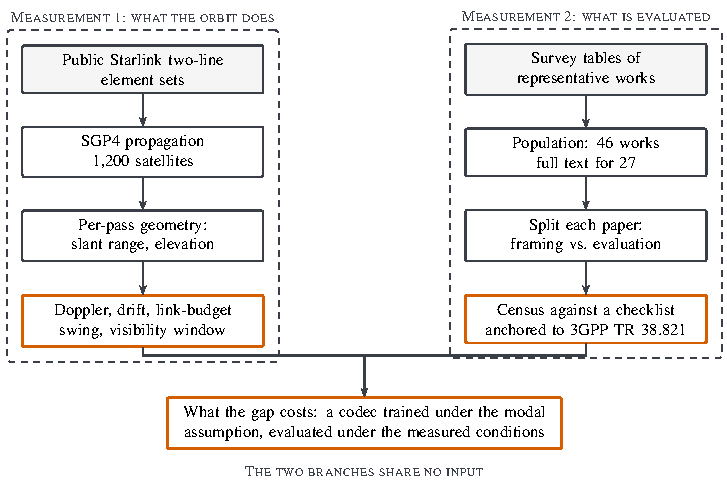
\includegraphics[width=\textwidth]{../figures/out/fig1-protocol.pdf}
\caption{The audit. The two measurements are independent: the orbital side never consults the
literature and the census never consults the orbit. They meet only in
Section~\ref{sec:cost}, where the conditions measured on the left are applied to a codec
trained under the assumption counted on the right.}
\label{fig:protocol}
\end{figure}

% =====================================================================
\section{Background}

\subsection{Why non-terrestrial links are said to be different}

A satellite in low Earth orbit moves at roughly $7.5$~km/s relative to the ground, which is the
origin of every constraint in the list above. Motion at that speed produces a Doppler shift
proportional to the carrier frequency, so a link that is untroubled at S-band becomes demanding
at Ka-band. It also bounds the time a given satellite is usable, since a pass ends when the
elevation angle falls below the minimum the link budget supports. And because free-space path
loss depends on slant range, which varies over the pass, the received power is not constant even
in the absence of fading.

These quantities are geometric. They follow from orbital elements, a ground station position and
a carrier frequency, and they can be computed rather than assumed. Section~\ref{sec:orbit} does
so, which is what allows the rest of the paper to speak about magnitudes instead of adjectives.

\subsection{Semantic communication and its evaluation}

Learned joint source-channel coding maps a source directly to channel symbols with a neural
encoder and reconstructs it with a neural decoder, trained end to end through a differentiable
channel~\cite{bourtsoulatze2019deepjscc}. The shift of objective from reproducing symbols to
preserving meaning is a departure from the classical formulation~\cite{shannon1948} and is set
out in~\cite{gunduz2023beyondbits}. The channel is therefore not an external assumption but a component of the training
objective, which is why the choice of channel model has consequences that reach beyond the
reported numbers: a codec learns to invert the impairments it is trained against and has no
reason to handle those it never saw.

Evaluation practice in the area has begun to receive attention from the metric side, asking how
semantic success should be defined and measured across modalities and tasks~\cite{metrics2026}. The present paper is
complementary and asks about conditions rather than metrics: given any metric, under what channel
was it computed.

\subsection{Audits as a genre}

Reassessments that re-run a body of work under stricter conditions have an established place in
networking. They have found reported gains in traffic classification that arose from dataset-specific
shortcuts rather than task semantics~\cite{shortcuts2026}, and reality checks in adjacent areas
have been published even when the reassessed method loses~\cite{spadari2025realitycheck}, because the contribution is the evaluation
protocol rather than a new mechanism. This paper follows that genre. Its contribution is a
protocol, a measurement of what the protocol is measuring against, and a released harness.

% =====================================================================
\section{The audit protocol}
\label{sec:protocol}

\subsection{Population}

The population is the set of works a recent survey of semantic communication for non-terrestrial
networks~\cite{survey2026ntnsemcom} lists in its representative-works tables, covering satellite,
aerial and integrated scenarios. Using a survey as the sampling frame is a convenience sample and we treat it as one,
with the consequences discussed in Section~\ref{sec:threats}. It has one property that outweighs
the cost: the pairing between an NTN limitation and the works said to address it is made by the
field rather than by us, so the audit tests a claim the community has already put in print.

The tables list \numPop{} distinct works~\cite{bhattacharjee2024r113,cao2025r94,chou2024r154,hassan2024r95,huang2024r112,huang2026r117,huang2026r165,jiang2024r93,joshi2026r179,kang2022r180,lin2023r116,liu2026r100,nguyen2024r115,nguyen2025r104,nguyenkha2026r170,qiu2025r200,razlighi2026r118,sankara2026r186,siyun2025r191,song2024r102,tian2026r178,uysal2024r108,yin2025r203,zeng2026r81,zhang2024r161,zhao2024r114,zheng2026r190}. Full text could be obtained for \numFull{}, which is
\numFullPct\% of the population; the remaining \numNotFull{} are counted as not auditable rather
than guessed at, since a work whose evaluation section cannot be read is a fact about the
accessibility of the literature and not a gap to be filled by inference.

\subsection{Checklist}

Table~\ref{tab:checklist} states the checklist: \numChecklist{} items covering the physical
effects an NTN evaluation could instantiate and the channel models it could use, each with the
source it is anchored to. \numFromSurvey{} of the items restate structural constraints the
field's own survey names, the standardised-model item points at the 3GPP studies, and the
remainder are protocol conventions rather than physical effects. Two design decisions matter. The effects are
those the field's own survey names as structural NTN constraints, and the channel-model entries
follow the 3GPP non-terrestrial studies~\cite{tr38811,tr38821}, so neither list is ours. And the checklist is deliberately
about \emph{conditions of evaluation}, not about quality: a work that evaluates over additive
white Gaussian noise is not thereby wrong, it is evaluated under a stated condition, and the
audit records which condition.

\subsection{Coding, and where a claim counts}

The instrument is a distinction between two regions of a paper. A sentence about Doppler in an
introduction or a related-work section states a motivation. The same sentence in a simulation
setup or results section is evidence that the evaluation instantiates the effect. Every paper is
therefore split at the first heading that begins its evaluation, and every checklist item is
coded separately for the region before and the region after.

The extraction step returns sentences rather than verdicts. For each work and each checklist
item, the harness collects the sentences that bear on the item, tagged by region, and a decision
is recorded against those sentences. The coding sheet released with this paper carries the
sentence behind every decision, so any individual judgement can be disputed without repeating
the collection.

\subsection{Testing the instrument before trusting it}

Two checklist items return zero across the whole population, and a zero is exactly where a
broken detector is indistinguishable from a finding. Three controls therefore run before any
zero is quoted. Sentences written the way papers actually write them must be caught, including
phrasings that avoid the obvious keyword. Near misses must be rejected, among them a mention of
3GPP that is not a channel model. And the detectors must demonstrably fire on the real corpus,
which rules out an empty-input failure in which every count is zero because nothing was read. All
three pass, and the controls are released as an executable script rather than described.

% =====================================================================
\section{What the orbit actually does}
\label{sec:orbit}

\subsection{Method}

A seeded sample of \numSats{} Starlink two-line element sets is propagated with
SGP4~\cite{vallado2006sgp4} over
\numPasses{} passes at four ground stations spanning $0$ to $65$ degrees of latitude. For each
pass we record slant range, elevation, one-way delay, the Doppler shift implied by the range
rate at S-band and Ka-band, its time derivative, and the free-space path loss.

\paragraph{Only geometry, deliberately.}
We compute free-space path loss and nothing else. Antenna pattern roll-off across a pass,
atmospheric and rain attenuation and receiver noise figure all \emph{add} variation rather than
removing it, so the swing reported here is a lower bound on how much the link budget moves. A
lower bound requires no contested modelling, and the argument of this paper needs only a lower
bound.

\subsection{Results}

Figure~\ref{fig:orbital} shows the three distributions that matter and
Table~\ref{tab:stations} reports them per station. Peak Doppler at Ka-band has a median of
\numDopKaMed~kHz and reaches \numDopKaMax~kHz, which is the literal content of the phrase
``hundreds of kilohertz'' that motivates the area. At S-band the same passes give
\numDopS~kHz. The drift has a median of \numDopRate~kHz/s and a maximum of
\numDopRateMax~kHz/s, so the shift is not a constant offset that a single estimate removes. The
geometric term of the link budget sweeps a median of \numFsplMed~dB and up to \numFsplMax~dB
over a median visibility window of \numDurMed~s, and one-way delay reaches \numOwd~ms.

\begin{figure}[t]
\centering
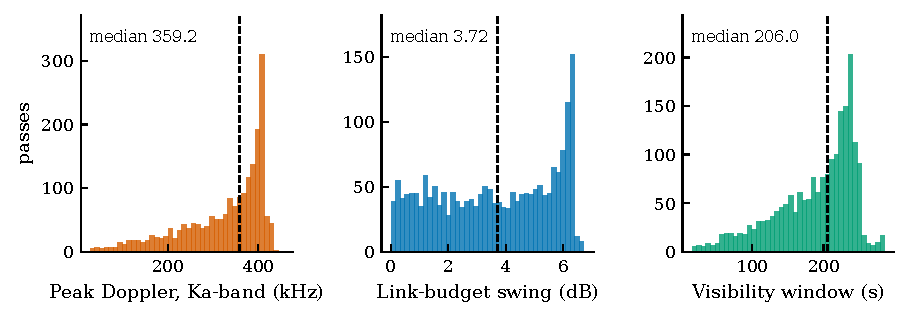
\includegraphics[width=\textwidth]{../figures/out/fig2-orbital.pdf}
\caption{Distributions over \numPassesStation{} passes at one station with a minimum elevation of
$25^\circ$: peak Doppler shift at Ka-band, the swing of the geometric link-budget term across a
pass, and the visibility window. Dashed lines mark medians. The bimodality of the centre panel reflects the difference
between overhead passes, which sweep the full range of slant range, and grazing passes, which
do not.}
\label{fig:orbital}
\end{figure}

\begin{table}[t]
\centering
\caption{Medians per ground station at a minimum elevation of $25^\circ$. The quantities differ
by at most \numDopSpread~kHz in Doppler across $65$ degrees of latitude, so they are properties
of the orbital shell rather than of a chosen site.}
\label{tab:stations}
\begin{tabular}{lrrrrr}
\toprule
Ground station & Lat. ($^\circ$) & Passes & Window (s) & Swing (dB) & Doppler (kHz) \\
\midrule
Da Nang & 16.0 & 1,978 & 206.0 & 3.72 & 359.2 \\
Equator & 0.0 & 1,878 & 205.5 & 3.67 & 356.3 \\
Mid-lat & 45.0 & 3,663 & 200.5 & 3.61 & 354.5 \\
High-lat & 65.0 & 927 & 215.0 & 3.87 & 370.1 \\
\bottomrule
\end{tabular}

\end{table}

\subsection{One pass, in detail}

Figure~\ref{fig:pass} follows a single pass, and the pass is chosen by a stated rule rather than
for appearance: it is the one whose maximum elevation lies closest to the median of the
distribution. Over its \numPassDur~s the Ka-band shift runs from \numPassDopLo~kHz to
\numPassDopHi~kHz, an excursion of \numPassDopSpan~kHz that passes through zero at closest
approach, so the sign of the offset reverses within a single contact. The shaded band marks a
one-second transmission block at the same scale. Its width against the pass is the visual form
of the two results of this section: nothing of consequence happens to the link budget inside the
block, and a great deal happens across the pass that contains it.

\begin{figure}[t]
\centering
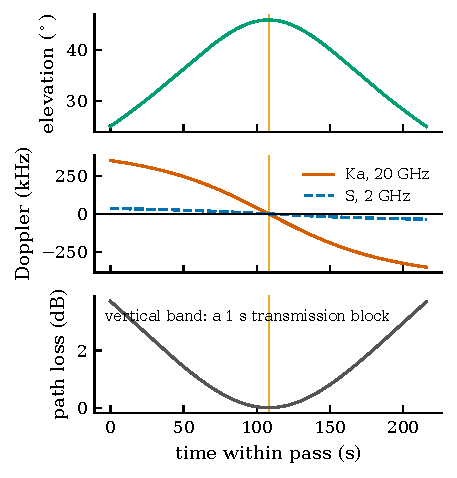
\includegraphics[width=0.65\textwidth]{../figures/out/fig3-pass.pdf}
\caption{One pass of \numPassSat{} over the station, reaching \numPassElMax$^\circ$. The
selection rule is stated in the text and in the released code. Path loss is plotted relative to
its minimum.}
\label{fig:pass}
\end{figure}

\subsection{Sensitivity to the elevation threshold}

The minimum elevation a link supports is a design choice, and it moves every quantity above.
Figure~\ref{fig:elev} and Table~\ref{tab:orbital} report the three thresholds the 3GPP studies
use. Raising the threshold from $10^\circ$ to $30^\circ$ cuts the number of usable passes at
one station from \numPassTen{} to \numPassThirty{} per day while shortening the window, so a
stricter threshold buys a better link at the cost of contact time. The Doppler extremes fall
because the geometry excludes the low-elevation part of the pass where the range rate is
largest, but they remain in the hundreds of kilohertz at every threshold.

\begin{figure}[t]
\centering
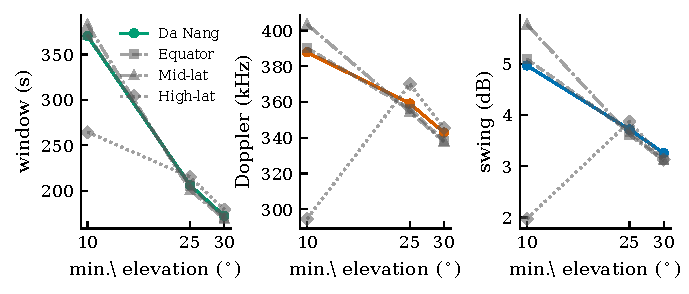
\includegraphics[width=\textwidth]{../figures/out/fig4-elevation.pdf}
\caption{Medians of the same three quantities, visibility window, peak Ka-band Doppler and
link-budget swing, against the minimum elevation threshold, for four stations. The station used
elsewhere in this paper is drawn in colour and the others in grey; the curves lie close together,
which is the same shell property Table~\ref{tab:stations} reports.}
\label{fig:elev}
\end{figure}

\begin{table}[t]
\centering
\caption{Full statistics at one station for the three elevation thresholds. Link-budget figures
are the geometric term only and are therefore lower bounds.}
\label{tab:orbital}
\begin{tabular}{lrrrrrr}
\toprule
& \multicolumn{2}{c}{$10^\circ$} & \multicolumn{2}{c}{$25^\circ$} & \multicolumn{2}{c}{$30^\circ$} \\
\cmidrule(lr){2-3}\cmidrule(lr){4-5}\cmidrule(lr){6-7}
Quantity & median & max & median & max & median & max \\
\midrule
Visibility window (s) & 370.2 & 502.0 & 206.0 & 285.5 & 172.0 & 241.0 \\
One-way delay (ms) & 5.41 & 6.26 & 3.25 & 3.90 & 2.86 & 3.45 \\
Peak Doppler, S-band (kHz) & 38.8 & 49.7 & 35.9 & 45.6 & 34.3 & 43.4 \\
Peak Doppler, Ka-band (kHz) & 387.8 & 497.0 & 359.2 & 455.5 & 342.9 & 433.5 \\
Doppler drift, Ka (kHz/s) & 3.66 & 16.88 & 5.36 & 16.88 & 5.73 & 16.88 \\
Link-budget swing (dB) & 4.97 & 12.15 & 3.72 & 6.72 & 3.26 & 5.45 \\
Link-budget slew (dB/s) & 0.034 & 0.143 & 0.049 & 0.143 & 0.052 & 0.143 \\
\bottomrule
\end{tabular}

\end{table}

\subsection{The result that runs against the audit}

The rate at which the link budget moves has a median of \numSlew~dB/s. Over a one-second
transmission the signal-to-noise ratio therefore shifts by well under a tenth of a decibel, and
over ten seconds by \numSlewTen~dB. The common practice of holding the signal-to-noise ratio
fixed within a transmission block is sound, and an audit that attacked it would be attacking the
wrong thing.

What this leaves is a different question, and it is the one Section~\ref{sec:cost} asks. The
sweep is small per second but not small per pass. A codec trained at one operating point is
deployed across a window of \numDurMed~s over which the geometric term alone moves
\numFsplMed~dB.

% =====================================================================
\section{What the literature actually evaluates}
\label{sec:census}

Figure~\ref{fig:census} and Table~\ref{tab:census} report the census over the \numCoded{} works
for which full text was available and an evaluation section could be located.

\paragraph{Channel models.}
Additive white Gaussian noise is the modal choice, present in the evaluation of
\numEvCHAWGN{} works. Statistical fading appears in \numEvCHFADING{}. A standardised
non-terrestrial channel model appears in \numEvCHGPP{}. No work in the population drives its
channel from orbital data: the count for two-line elements, SGP4, ephemeris or an equivalent
propagation tool is \numEvCHTRACE{}.

\paragraph{Effects.}
Doppler appears in the evaluation of \numEvDOPPLER{} works and in the framing of
\numInDOPPLER{}. Its time-varying component appears in \numEvDOPPLERRATE{}. Elevation-dependent
loss appears in \numEvPATHLOSSELEV{}, propagation delay in \numEvDELAY{}, a finite visibility
window in \numEvVISIBILITY{}, and an on-board compute limit in \numEvONBOARD{}.

\paragraph{Reading the two zeros.}
The zeros for time-varying Doppler and for orbital traces are measurements, not silence: the
controls of Section~\ref{sec:protocol} establish that the detectors catch the relevant phrasings
and do fire elsewhere in the same corpus. Read against Section~\ref{sec:orbit}, they say that the
drift the orbit produces, up to \numDopRateMax~kHz/s, is instantiated by no evaluation in the
population, and that no evaluation is driven by the geometry that produces it.

\paragraph{The structure behind the counts.}
Figure~\ref{fig:matrix} resolves the census to individual works. No evaluation in the population
instantiates more than \numMaxCover{} of the \numChecklist{} items, and \numZeroCover{} works
instantiate none of them. The two empty rows are the zeros discussed above, and seeing them as
rows rather than as bars makes clear that they are not the result of one or two works dominating
a count.

\paragraph{A second source describes the same works.}
The survey's own channel-consideration column is an independent record of what each work
considers, so it can be compared against what the evaluation sections contain.
Table~\ref{tab:agreement} does that for the \numAgrN{} works where both are available. Two
things follow, and the first is not a criticism. The column is a phrase of a few words and cannot
enumerate an evaluation, so the entries naming fewer items than the evaluations contain is
expected. What is informative is what the entries name at all: across \numAgrN{} works they
name \numAgrNamedTot{} checklist items in total, because most entries describe an architecture
or a topology rather than a propagation environment. The column is the closest thing the
literature has to a record of channel realism, and it is not one. In \numAgrExtra{} case the
comparison runs the other way, with the column naming an effect the evaluation section does not
contain.

\begin{table}[t]
\centering
\caption{The survey's channel-consideration entry against the evaluation sections, for the
\numAgrN{} works where both could be read. ``Named'' counts checklist items the entry mentions,
``In eval.'' counts items the evaluation instantiates.}
\label{tab:agreement}
\begin{tabular}{rlccl}
\toprule
Work & Survey's channel entry & Named & In eval. & Named but absent \\
\midrule
{[95]} & EO downlink, visibility window & 1 & 0 & Finite visibility window \\
{[81]} & Multi-hop ISL routing & 0 & 2 & --- \\
{[93]} & Adaptive encoder-decoder & 0 & 6 & --- \\
{[94]} & SNR-aware codec & 0 & 4 & --- \\
{[100]} & Doppler, weather fading & 1 & 6 & --- \\
{[104]} & Hierarchical FL & 0 & 5 & --- \\
{[113]} & On-board sparse encoder & 0 & 1 & --- \\
{[115]} & Multi-gateway hops, SNR-aware & 0 & 4 & --- \\
{[116]} & Cooperative relaying & 0 & 1 & --- \\
{[117]} & Semantic forwarding & 0 & 0 & --- \\
{[118]} & Task-clustered FL & 0 & 1 & --- \\
{[154]} & Inter-satellite links & 0 & 7 & --- \\
{[161]} & Satellite interference & 0 & 2 & --- \\
{[165]} & Direct Satellite Communication & 0 & 4 & --- \\
{[170]} & SNR-aware link & 0 & 4 & --- \\
\bottomrule
\end{tabular}

\end{table}

\begin{figure}[t]
\centering
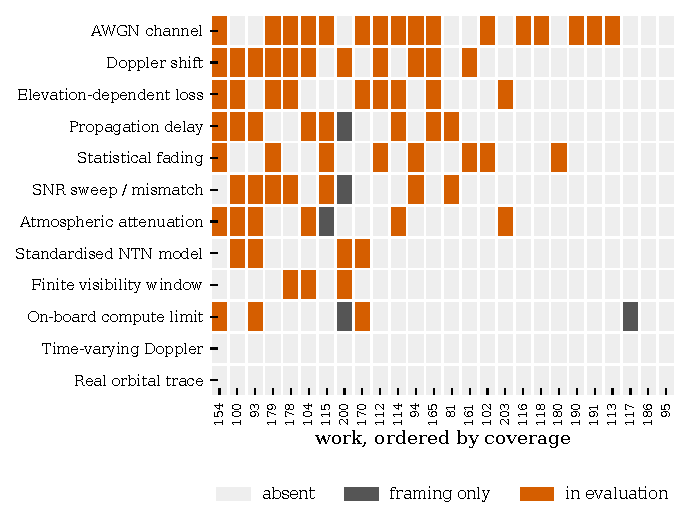
\includegraphics[width=\textwidth]{../figures/out/fig6-matrix.pdf}
\caption{Every codeable work against every checklist item, ordered by coverage. Grey marks an
effect that appears only while the problem is being motivated; orange marks one the evaluation
instantiates.}
\label{fig:matrix}
\end{figure}

\begin{figure}[t]
\centering
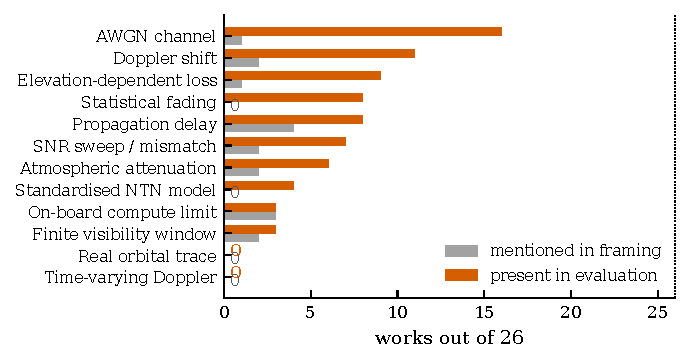
\includegraphics[width=0.62\textwidth]{../figures/out/fig5-census.pdf}
\caption{Where each effect appears, for the \numCoded{} codeable works. Grey counts works that
mention the effect only while motivating the problem; orange counts works whose evaluation
instantiates it. Zeros are labelled explicitly so that a measured zero is not read as a missing
bar.}
\label{fig:census}
\end{figure}

\begin{table}[t]
\centering
\caption{The checklist, with the source each item is anchored to. ``Survey'' items restate
structural constraints named by the field's own survey, ``3GPP'' points at the non-terrestrial
channel studies, ``Orbit'' follows from orbital mechanics, and ``Protocol'' items are evaluation
conventions rather than physical effects.}
\label{tab:checklist}
\begin{tabular}{llp{62mm}}
\toprule
Item & Anchor & What the item asks the evaluation to instantiate \\
\midrule
Doppler shift & Survey & Large and time-varying Doppler shift \\
Time-varying Doppler & Survey & the time-varying component of the same constraint \\
Propagation delay & Survey & Long propagation delay \\
Elevation-dependent loss & Survey & Severe and time-varying path loss \\
Finite visibility window & Survey & Intermittent connectivity, short visibility windows \\
Atmospheric attenuation & Survey & Atmospheric and weather attenuation \\
On-board compute limit & Survey & On-board size, weight and power limits \\
AWGN channel & Protocol & conventional terrestrial reference channel \\
Statistical fading & Protocol & conventional statistical fading channel \\
Standardised NTN model & 3GPP & TR 38.811 / TR 38.821 non-terrestrial channel \\
Real orbital trace & Orbit & channel driven by propagated orbital elements \\
SNR sweep / mismatch & Protocol & operating range rather than operating point \\
\bottomrule
\end{tabular}

\end{table}

\begin{table}[t]
\centering
\caption{Census over \numCoded{} works. ``Framing'' counts appearances before the evaluation
section, ``Evaluation'' counts appearances within it. A work may appear in both columns.}
\label{tab:census}
\begin{tabular}{llrr}
\toprule
Code & NTN effect or channel model & Framing & Evaluation \\
\midrule
\texttt{CH\_AWGN} & AWGN channel & 1 & 16 \\
\texttt{DOPPLER} & Doppler shift & 2 & 11 \\
\texttt{PATHLOSS\_ELEV} & Elevation-dependent loss & 1 & 9 \\
\texttt{CH\_FADING} & Statistical fading & 0 & 8 \\
\texttt{DELAY} & Propagation delay & 4 & 8 \\
\texttt{SNR\_SWEEP} & SNR sweep / mismatch & 2 & 7 \\
\texttt{ATMOS} & Atmospheric attenuation & 2 & 6 \\
\texttt{CH\_3GPP} & Standardised NTN model & 0 & 4 \\
\texttt{ONBOARD} & On-board compute limit & 3 & 3 \\
\texttt{VISIBILITY} & Finite visibility window & 2 & 3 \\
\texttt{CH\_TRACE} & Real orbital trace & 0 & 0 \\
\texttt{DOPPLER\_RATE} & Time-varying Doppler & 0 & 0 \\
\bottomrule
\end{tabular}

\end{table}

% =====================================================================
\section{What the gap costs}
\label{sec:cost}

The census establishes what the population evaluates and Section~\ref{sec:orbit} establishes what
the orbit does. This section joins them by taking the modal assumption of the population, an
additive white Gaussian noise channel at a single signal-to-noise ratio, and asking what happens
to a codec trained under it when the conditions of Section~\ref{sec:orbit} are applied.

\subsection{Setup}

A convolutional joint source-channel codec~\cite{bourtsoulatze2019deepjscc} is trained end to
end through a differentiable complex additive white Gaussian noise channel on a standard image
benchmark~\cite{krizhevsky2009cifar}. Two training regimes are compared. The first
fixes the signal-to-noise ratio during training, which is the modal practice in the population.
The second randomises it, together with a residual frequency offset, over the ranges
Section~\ref{sec:orbit} measured. The second regime is included so that the paper reports a
remedy rather than only a deficiency, and so that the cost of the gap can be separated from the
cost of fixing it.

\paragraph{The evaluation range is not chosen by us.}
The sweep spans the link-budget swing measured in Section~\ref{sec:orbit} rather than a range
picked for effect, and because that swing excludes antenna pattern and atmospherics it is the
conservative end of what a deployed codec would see.

\paragraph{Residual offset, not raw Doppler.}
No deployed system leaves \numDopKaMed~kHz uncompensated, so evaluating at raw Doppler would be a
straw man. We parameterise instead by the normalised residual offset
$\varepsilon = f_{\mathrm{res}}/R_s$, the phase advance added per channel use, which avoids
committing to a symbol rate that no work in the population states. A reader substitutes their own
$R_s$ to locate their operating point: at the median Ka-band shift of \numDopKaMed~kHz and a
symbol rate of $10$~Msym/s, leaving one per cent of the shift uncorrected puts
$\varepsilon$ near $3.6\times10^{-4}$.

% =====================================================================
\section{Recommendations}

Three things follow, in decreasing order of confidence.

\textbf{State the channel, and state it in the units of the orbit.} An evaluation over additive
white Gaussian noise at a fixed signal-to-noise ratio is a legitimate experiment and this paper
does not argue otherwise. What is missing is the translation: at what elevation, at what point in
a pass, and under what residual frequency offset does the stated operating point sit. The
generator released here performs that translation from public orbital elements in a few lines.

\textbf{Report the operating range, not the operating point.} A visibility window of
\numDurMed~s over which the geometric term alone moves \numFsplMed~dB is the interval a deployed
codec must serve. Reporting a single number at the centre of that interval describes the best
case.

\textbf{Treat residual frequency offset as a swept parameter.} Doppler is compensated in practice
and no serious system leaves \numDopKaMed~kHz uncorrected. What matters is the residual, and
because the tolerable residual is a property of the codec rather than of the link, it belongs in
the evaluation of the codec.

% =====================================================================
\section{Threats to validity}
\label{sec:threats}

\textbf{One survey is one sampling frame.} The population is a convenience sample drawn from a
single recent survey. It is not a systematic review, and a work absent from that survey is absent
here. What the sample buys is that the pairing between limitation and work is the field's rather
than ours, which is the specific claim under test.

\textbf{Two fifths of the population could not be read.} Full text was obtained for \numFull{} of
\numPop{} works. The \numNotFull{} that could not be obtained may well instantiate effects the
audit does not credit them with. They are excluded from every count rather than assumed absent,
and the denominator \numCoded{} is stated wherever a proportion appears.

\textbf{Absence of a phrase is not absence of a model.} The census detects the vocabulary in
which an effect is normally described. A work could model time-varying Doppler without using any
of the phrasings the controls test. This is why the coding sheet is released with the sentences
attached rather than only the counts.

\textbf{The orbital measurement is one constellation.} All figures come from Starlink elements at
one epoch. Other shells at other altitudes will shift the numbers, though the geometry that
produces them does not change in kind.

\textbf{Free-space path loss is a lower bound, not the link budget.} The swing reported here
excludes antenna pattern, atmospherics and noise figure. Every one of them widens the range, so
the direction of the bound is known even though its tightness is not.

% =====================================================================
\section{Conclusion}

Surveys of semantic communication for non-terrestrial networks map each constraint of the
satellite link onto the works said to address it. Measuring both sides of that mapping shows
where it is load-bearing and where it is not. The orbit produces a Doppler shift with a median
peak of \numDopKaMed~kHz drifting at up to \numDopRateMax~kHz/s and a link budget that sweeps
\numFsplMed~dB across a \numDurMed~s window. Of the \numCoded{} works of Section~\ref{sec:census} that could be read and coded,
\numEvCHAWGN{} evaluate over additive white Gaussian noise, \numEvCHGPP{} use a standardised
non-terrestrial model, and none instantiates either the drift or the geometry that produces it.

The reading is not that this work is unsound. It is that the case for semantic communication in
non-terrestrial networks currently rests on evaluations conducted under terrestrial conditions,
and that closing the distance is cheap: the orbital elements are public, the propagation is a
library call, and the harness that connects them to an existing codec is released with this
paper.

\section*{Data availability}
The checklist, the coding sheet with the sentence justifying every decision, the orbital
generator, the detector controls and the evaluation harness are released.

\bibliographystyle{elsarticle-num}
\bibliography{refs,refs-population}

\end{document}
